\documentclass[
    % 12pt,
    % onehalfspacing,
    % secnum,
    % twocolumn,
]
{thepaper}


\usepackage{amsmath}
\usepackage{lipsum}
\usepackage{mhchem} % For chemical notation
\usepackage{siunitx}    % For SI units
\usepackage{gensymb}    % Symbols
\usepackage[misc]{ifsym} % For the \Letter symbol
\usepackage{tabularx}   % For making Knitr tables compatible
\usepackage{multirow}
\usepackage{wrapfig}
\usepackage{gensymb}
\usepackage{caption}

\bibliographystyle{aps}


%%%%%%%%%%%%%%%%%%%%%%%%%%%%%%%%%%%%%
%%%         TITLE PAGE
%%%%%%%%%%%%%%%%%%%%%%%%%%%%%%%%%%%%%
\title{My Awesome Template for Research Article}

\author[1]{Minjoon Hong}
\author[2, *]{Co-author}\corrauth{example@example.com}

% Affiliations
\affil[1]{School of Life Sciences, University of Sussex}
\affil[2]{University of Somewhere}

\begin{document}

\newcommand{\abs}{\lipsum[1]}
% \twocolumn[
    \begin{@twocolumnfalse}
        \maketitle
        \begin{abstract}
            \abs
        \end{abstract}
        \keywords{Keyword 1, Keyword 2, Keyword 3}
    \end{@twocolumnfalse}
% ]

%%%%%%%%%%%%%%%%%%%%%%%%%%%%%%%%%%%%%
%%%         MAIN TEXT
%%%%%%%%%%%%%%%%%%%%%%%%%%%%%%%%%%%%%
\section{Section}
Section is the top level of the hierarchy.

\subsection{Subsection}
Subsection is the second level of the hierarchy.

\subsubsection{Subsubsection}
Subsubsection is the third level of the hierarchy.

\lipsum[2-6]


\section{Examples}

\subsection{Figures}

\begin{figure}[!htbp]
    \centering
    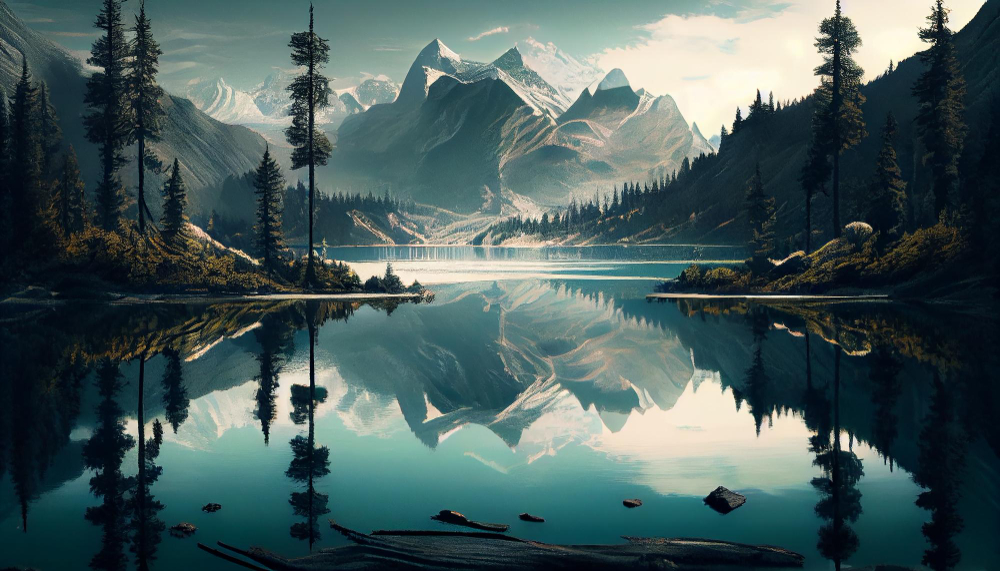
\includegraphics[width=0.5\linewidth]{src/images/example.jpg}
    \caption{This is a caption.}
    \label{fig:1}
\end{figure}



\subsection{Tables}

\begin{table}[h!]
    \centering
    \begin{tabular}{c c c c} 
     \hline
     Col1 & Col2 & Col2 & Col3 \\ 
     \hline
     1 & 6 & 87837 & 787 \\ 
     2 & 7 & 78 & 5415 \\
     3 & 545 & 778 & 7507 \\
     4 & 545 & 18744 & 7560 \\
     5 & 88 & 788 & 6344 \\
     \hline
    \end{tabular}
    \caption{Table to test captions and labels.}
    \label{table:1}
\end{table}

\subsection{References}
You can cite papers like this.\cite{neese2018}. To cite multiple papers at once, you can do this.\cite{neese2018,example2}


\bibliography{main}
\end{document}
